\chapter{State of the Art}
\label{ch:state_of_the_art}

\begin{figure}[h]
    \centering
    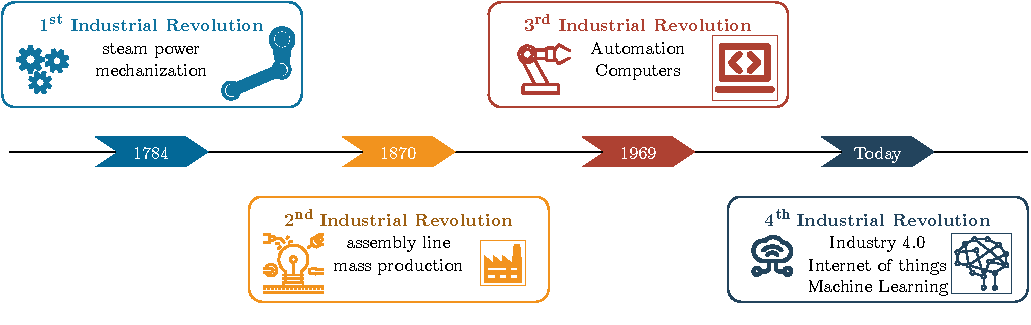
\includegraphics[width=\textwidth]{images/StateArt/Industry40.pdf}
    \caption{Industrial revolutions}
    \label{fig:ind40}    
\end{figure}

The invention of the modern steam engine in the $18^{th}$ century marked the beginning of the first industrial revolution. The second industrial revolution, in the $19^{th}$ century, was characterized by the introduction of mass production and the assembly line. The introduction of computers and automation in factories, in the $20^{th}$ century, enabled the third industrial revolution. Nowadays, we are currently living in the $4^{th}$ industrial revolution, that embraces the industry $4.0$ vision. State-of-the-art industries have small decentralized smart networks that make decisions autonomously. This is possible thanks to the \emph{Internet of Things} (\gls{iot}), smart sensors and actuators, and \emph{Big Data} analysis (\autoref{fig:ind40}). 
The data to be monitored varies \gls{wrt} the field of application. The most common are \cite{State_Art_Coanda_2020}:
\begin{itemize}
    \item Vibration Analysis - Efficient method for detecting issues in rotating equipment.
    \item Acoustic Analysis - Detects or monitors cracks in pipes and other structures.
    \item Lubrication Oils Analysis - Analyzes particles in oils to assess component wear.
    \item Particle Analysis in Working Environment - Applied to equipment operating in fluid environments.
    \item Corrosive Analysis - Ultrasound measurements to determine corrosion in various structures.
    \item Thermal Analysis - Identifies overheating in mechanical and electrical systems.
    \item Performance Analysis - Efficient technique for pinpointing operational problems in the system.
\end{itemize}



\paragraph{Standard terminology}
\begin{figure}
    \centering
    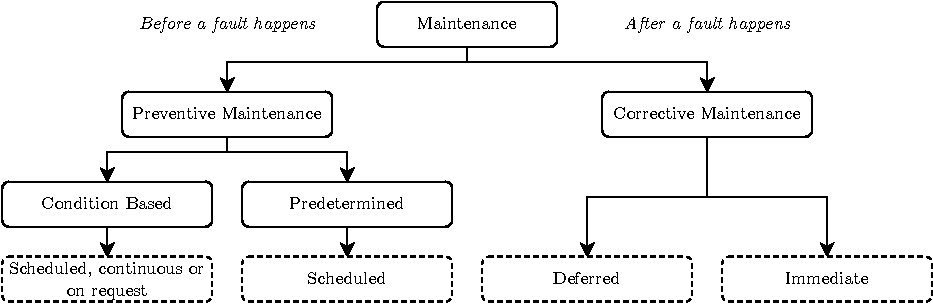
\includegraphics[width=\textwidth]{images/StateArt/EN_classification.drawio.pdf}
    \caption{Standard terminology for industrial maintenance \cite{rastegari2017condition}}
    \label{fig:standard_terminology}
\end{figure}

A standard terminology used for industrial maintenance is provided by the European committee for standardization with the standard \texttt{EN13306:2018} \cite{EN13306:2018}. The terminology is summarized in \autoref{fig:standard_terminology}. The most advanced maintenance technique family is \textbf{\gls{glo:conditionbasedmaintenance}}. This category includes the most modern \textbf{\gls{glo:predictivemaintenance}}. Note that the definition does not imply that the \quoted{monitoring} of the system must be continuous, it may also be scheduled or not even scheduled and performed both manually or by a program.

The standard also defines what \textbf{\gls{glo:onlinemaintenance}} and \textbf{\gls{glo:onistemaintenance}}. All these definitions are reported in the {glossary}.


\paragraph{\gls{rm} vs \gls{pm}}
\begin{figure}
    \centering
    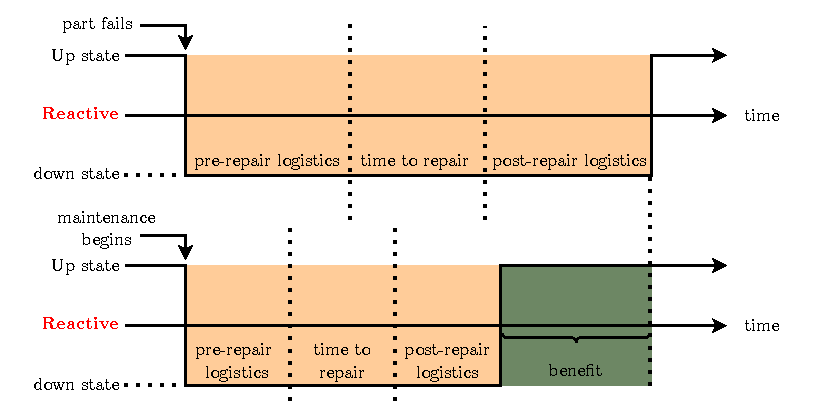
\includegraphics[width=\textwidth]{images/StateArt/lost_opportunities.pdf}
    \caption{Downtime comparison (\gls{rm} and \gls{pm})}
    \label{fig:lost_opportunities}
\end{figure}

As anticipated in the introduction, the two main approaches are \textbf{Reactive Maintenance} (\gls{aka} \gls{glo:correctivemaintenance}), which restores system functionality, and \textbf{Proactive Maintenance} (\gls{aka} \gls{glo:preventivemaintenance}), which preserves system functionality \cite{Rely_maint_book}.

The former approach leads to very high downtime \gls{wrt} the latter \cite{NIST}. For all the time a system is down, the company forfeits the opportunity to make a profit. This is called \emph{lost opportunity cost}. In reality, the total costs of downtime are even higher, because there are other costs associated with labor overhead and materials \cite{Lost_Opport_Cost}. The second approach optimizes both the pre-repair and post-repair logistics and, acting before the failure, can reduce also the total downtime. A qualitative diagram of these benefits is shown in \autoref{fig:lost_opportunities}. Other than the downtime, a more complete comparison between the advantages and disadvantages of the two approaches is shown in \autoref{tab:PM_vs_RM}.

% \usepackage{array}
% \usepackage{booktabs}


\begin{table}
    \centering
    \caption{Advantages and disadvantages of \gls{rm} and \gls{pm} maintenance \cite{Lost_Opport_Cost}}
    \resizebox{0.999999\textwidth}{!}{%
    \begin{tabular}{>{\hspace{0pt}}m{0.2\linewidth}>{\hspace{0pt}}m{0.344\linewidth}>{\hspace{0pt}}m{0.39\linewidth}} 
    \toprule
    \textbf{Maintenance} & \textbf{Advantages}                                                                                                                                                                                                                                                                                                                                                                                                                                                                                                                                                                                                                                                                                                                                                                                                                                                                                                                                  & \textbf{Disadvantages}                                                                                                                                                                                                               \\ 
    \hline
    Reactive             & \begin{tabular}{@{\labelitemi\hspace{\dimexpr\labelsep+0.5\tabcolsep}}l@{}}low setup cost\\easy to setup\end{tabular}                                                                                                                                                                                                                                                                                                                                                                                                                                                                                                                                                                                                                                                                                                                                                                                                                                & \begin{tabular}{@{\labelitemi\hspace{\dimexpr\labelsep+0.5\tabcolsep}}l@{}}unscheduled downtime\\increased labour costs\\unoptimized resources\\\begin{tabular}[c]{@{}l@{}}Increased manufacturing\\costs\end{tabular}\end{tabular}  \\ 
    \hline
    Proactive            & \begin{tabular}{@{}l@{}}{\labelitemi}\hspace{\dimexpr\labelsep+0.5\tabcolsep}\begin{tabular}[c]{@{}l@{}}increases system\\availability\end{tabular}\\{\labelitemi}\hspace{\dimexpr\labelsep+0.5\tabcolsep}\begin{tabular}[c]{@{}l@{}}minimizes logistical\\downtime\end{tabular}\\{\labelitemi}\hspace{\dimexpr\labelsep+0.5\tabcolsep}\begin{tabular}[c]{@{}l@{}}reduces unscheduled\\downtime\end{tabular}\\{\labelitemi}\hspace{\dimexpr\labelsep+0.5\tabcolsep}~decreases costs\\\hspace{0.5\leftmargin}{\labelitemii}\hspace{\dimexpr\labelsep+0.5\tabcolsep}optimizes parts\\\hspace{0.5\leftmargin}{\labelitemii}\hspace{\dimexpr\labelsep+0.5\tabcolsep}optimizes labour\\{\labelitemi}\hspace{\dimexpr\labelsep+0.5\tabcolsep}\begin{tabular}[c]{@{}l@{}}maintenance events\\planned\end{tabular}\\{\labelitemi}\hspace{\dimexpr\labelsep+0.5\tabcolsep}\begin{tabular}[c]{@{}l@{}}optimize logistical\\support~~\end{tabular}\end{tabular} & \begin{tabular}{@{\labelitemi\hspace{\dimexpr\labelsep+0.5\tabcolsep}}l@{}}high setup cost\\\begin{tabular}[c]{@{}l@{}}savings not seen\\immediately\end{tabular}\\not feasible forall equipment~\end{tabular}                       \\
    \bottomrule
    \end{tabular}
    }
    \end{table}

\paragraph{Passive vs Active maintenance}
\gls{pdm} techniques can be divided also into \emph{passive} and \emph{active}. The former uses existing sensors or adds new sensors to the system and these data are just analyzed. The latter, instead, uses actuators to perturb the system and then analyzes the response. The former is more common because it is less expensive and less invasive. The latter, instead, is more accurate but its application is limited to special applications. The most common field of application of active \gls{pdm} is electrical systems, where the perturbation can be applied by injecting a current or a voltage \cite{State_Art_Hasemian_2011}.

In \cite{State_Art_Hasemian_2011}, the author proposes also, as an example of active \gls{pdm}, the use of the Loop Current Step Response (\gls{lcsr}) technique. In this test, an electrical signal in the form of a step change is sent to the sensor using a Wheatstone bridge, causing heating in the \gls{rtd} sensing element. The resulting exponential transient at the bridge output is analyzed to determine the \gls{rtd}'s response time. Beyond measuring response time, the \gls{lcsr} test can serve other purposes, such as detecting water levels in a pipe and ensuring the proper installation of temperature sensors in thermowells. Moreover, it aids in verifying timely responses to temperature changes and identifying potential degradation due to ageing.

\paragraph{Models of degradation}
In \cite{Pred_Maint_Tech_Grall}, the authors propose a decision model that optimizes the inspection schedule and replacement time to minimize the cost of failure and unavailability. This procedure is based on two variables: the \emph{replacement threshold} and the \emph{inspection schedule}. Most of the non \gls{cbm} policy can be emulated with specific values of these two variables. This is applied to gradually deteriorating single-unit systems. The degradation is simulated with a random model that also considers the time to perform maintenance for an arbitrary period.

Another approach for characterizing the degradation of a system is to use a stochastic model hypothesizing the use of an imperfect monitoring system. The data from the sensors are used to update the model with a Bayesian approach. The study is tested on simulated data that emulate a decaying system using Markov chains \cite{CURCURU2010989}\cite{GALANTE19981361}.

\paragraph{Cloud based \gls{pdm}}
A relatively new structure for \gls{pdm} is proposed in \cite{CloudBased_Wang}. The authors investigate a low-cost cloud-based paradigm based on the concept of \emph{mobile agents}, implemented in embedded Linux \gls{os} with open-source libraries. Compared to the traditional client-server paradigm, this approach enhances the scalability and flexibility of the system, reducing also the need for transmission of heavy raw data.

The concept of mobile agents used in this implementation can be resumed as autonomous software entities that can migrate from one host to another, carrying their data and state \cite{CUCURULL2009712}.

The authors of \cite{CloudBased_Wang} tested the mobile agent implementation with induction motors that exhibited different failure modes. For example, a motor with a broken rotor bar defect is analyzed, collecting raw current measurements, envelope analysis, and spectrum analysis. Spectrum analysis poses challenges in distinguishing healthy and faulty motor signals. However, a comparison of current envelopes reveals marked differences in energy concentration associated with broken rotor bar-related frequencies. The defects analyzed by the system are broken bar, bowed rotor, unbalanced rotor, stator winding defect, and defective bearing.

In the study \cite{calabreseRUL}, a cloud-based \gls{pdm} system is proposed and tested on a gearbox in a bench test. This study performs anomaly detection, fault detection, and \gls{rul} prediction. The \gls{rul} predictions are made by selecting a health indicator that is strongly correlated with the remaining life of the component.


\paragraph{Thermal imaging}
Yet another tool for detecting anomalies, mostly used for electrical devices, is gathering images of the device using an infrared camera. This method has the advantage of being noninvasive. The process of images is a whole discipline, in \cite{Thermography}, the authors use a multilayered perceptron \gls{mlp} to classify $11$~\gls{glo:feature}s of the images. They achieved $78\%$ accuracy using the \gls{mlp} alone, which has been enhanced to $84\%$ performing a graph cut.

\paragraph{Algorithms for \gls{pdm}}
To continue the overview of state-of-the-art \gls{pdm} techniques, we will now focus on the algorithms used to analyze the data. The two main categories of algorithms are \gls{glo:trad_ml} and \gls{glo:deep} (\gls{dl}).  The survey \cite{ran2019survey} provides a comprehensive overview of the most common algorithms used in \gls{pdm}, that we summarized in \autoref{tab:ML_algorithms}, that is a merge of \cite{ran2019survey},\cite{particlefilter},\cite{yang2018particle},\cite{VONBIRGELEN2018480} and \cite{lira2011adaptive}. \gls{ann}, \gls{dt}, \gls{svm}, \gls{knn}, \gls{pf}, \gls{art} and \gls{som} are \gls{ml} algorithms, while \gls{ae}, \gls{cnn}, \gls{rnn}, \gls{dbn}, \gls{gan}, \gls{tl} and \gls{dlr} are \gls{glo:deep} algorithms. The most common field of application of each algorithm is also reported in the table.


{
\small
\begin{longtblr}[
    caption = {\gls{ml} and \gls{dl} algorithms used in \gls{pdm} \cite{ran2019survey}},
    label = {tab:ML_algorithms},
  ]{
    cells = {t},
    hline{1,16} = {-}{0.08em},
  }
  \textbf{Algorithm} & \textbf{Acronym} & \textbf{Typical application}\\ \hline
  Artificial Neural Network & \gls{ann} & {\labelitemi\hspace{\dimexpr\labelsep+0.5\tabcolsep}fault diagnostic in bearings\\\labelitemi\hspace{\dimexpr\labelsep+0.5\tabcolsep}\gls{rul} predictions of bearings}\\
  Decision Tree & \gls{dt} & {\labelitemi\hspace{\dimexpr\labelsep+0.5\tabcolsep}fault diagnostic\\\phantom{\labelitemi}\hspace{\dimexpr\labelsep+0.5\tabcolsep}- grids\\\phantom{\labelitemi}\hspace{\dimexpr\labelsep+0.5\tabcolsep}- rail vehicles\\\phantom{\labelitemi}\hspace{\dimexpr\labelsep+0.5\tabcolsep}- bearings\\\phantom{\labelitemi}\hspace{\dimexpr\labelsep+0.5\tabcolsep}- hydraulics etc.\\\labelitemi\hspace{\dimexpr\labelsep+0.5\tabcolsep}fault prognosis\\\phantom{\labelitemi}\hspace{\dimexpr\labelsep+0.5\tabcolsep}- turbofans\\\phantom{\labelitemi}\hspace{\dimexpr\labelsep+0.5\tabcolsep}- batteries\\\phantom{\labelitemi}\hspace{\dimexpr\labelsep+0.5\tabcolsep}- mechanical systems etc.}\\
  Support Vector Machines & \gls{svm} & {\labelitemi\hspace{\dimexpr\labelsep+0.5\tabcolsep}fault diagnostic\\\phantom{\labelitemi}\hspace{\dimexpr\labelsep+0.5\tabcolsep}- rotation machinery\\\phantom{\labelitemi}\hspace{\dimexpr\labelsep+0.5\tabcolsep}- bearings\\\phantom{\labelitemi}\hspace{\dimexpr\labelsep+0.5\tabcolsep}- wind turbines etc.\\\labelitemi\hspace{\dimexpr\labelsep+0.5\tabcolsep}\gls{rul} predictions\\\phantom{\labelitemi}\hspace{\dimexpr\labelsep+0.5\tabcolsep}- batteries\\\phantom{\labelitemi}\hspace{\dimexpr\labelsep+0.5\tabcolsep}- bearings etc.}\\
  $k$-Nearest Neighbor & \gls{knn} & {\labelitemi\hspace{\dimexpr\labelsep+0.5\tabcolsep}fault diagnostic\\\labelitemi\hspace{\dimexpr\labelsep+0.5\tabcolsep}\gls{rul} prediction\\\labelitemi\hspace{\dimexpr\labelsep+0.5\tabcolsep}Early fault warning}\\
  Particle Filter \cite{particlefilter} & \gls{pf} & \labelitemi\hspace{\dimexpr\labelsep+0.5\tabcolsep}\gls{rul} in turbine application \cite{yang2018particle}\\
  Adaptive resonance theory & \gls{art} & {\labelitemi\hspace{\dimexpr\labelsep+0.5\tabcolsep}anomaly detection metal \\\phantom{\labelitemi}\hspace{\dimexpr\labelsep+0.5\tabcolsep}oxide surge arrester \cite{lira2011adaptive}}\\
  Self-Organizing Maps & \gls{som} & \labelitemi\hspace{\dimexpr\labelsep+0.5\tabcolsep}anomaly detection \cite{VONBIRGELEN2018480}\\
  Auto-Encoder & \gls{ae} & {\labelitemi\hspace{\dimexpr\labelsep+0.5\tabcolsep}feature extraction\\\labelitemi\hspace{\dimexpr\labelsep+0.5\tabcolsep}data fusion\\\labelitemi\hspace{\dimexpr\labelsep+0.5\tabcolsep}fault diagnostic\\\labelitemi\hspace{\dimexpr\labelsep+0.5\tabcolsep}degradation estimation\\\labelitemi\hspace{\dimexpr\labelsep+0.5\tabcolsep}\gls{rul} predictions}\\
  Convolutional Neural Network & \gls{cnn} & {\labelitemi\hspace{\dimexpr\labelsep+0.5\tabcolsep}(joint) fault diagnostic\\\labelitemi\hspace{\dimexpr\labelsep+0.5\tabcolsep}degradation estimation\\\labelitemi\hspace{\dimexpr\labelsep+0.5\tabcolsep}\gls{rul} predictions}\\
  Recurrent Neural Network & \gls{rnn} & {\labelitemi\hspace{\dimexpr\labelsep+0.5\tabcolsep}fault diagnostic\\\labelitemi\hspace{\dimexpr\labelsep+0.5\tabcolsep}\gls{rul} predictions\\\labelitemi\hspace{\dimexpr\labelsep+0.5\tabcolsep}health indicator}\\
  Deep Belief Network & \gls{dbn} & {\labelitemi\hspace{\dimexpr\labelsep+0.5\tabcolsep}feature extraction\\\labelitemi\hspace{\dimexpr\labelsep+0.5\tabcolsep}fault classification\\\labelitemi\hspace{\dimexpr\labelsep+0.5\tabcolsep}\gls{rul} predictions}\\
  Generative Adversarial Network & \gls{gan} & {\labelitemi\hspace{\dimexpr\labelsep+0.5\tabcolsep}class imbalance\\\labelitemi\hspace{\dimexpr\labelsep+0.5\tabcolsep}fault identification\\\labelitemi\hspace{\dimexpr\labelsep+0.5\tabcolsep}\gls{rul} predictions}\\
  Transfer Learning & \gls{tn} & {\labelitemi\hspace{\dimexpr\labelsep+0.5\tabcolsep}fault diagnosis\\\labelitemi\hspace{\dimexpr\labelsep+0.5\tabcolsep}\gls{rul} predictions}\\
  Deep Reinforcement Learning & \gls{dlr} & {\labelitemi\hspace{\dimexpr\labelsep+0.5\tabcolsep}decision making\\\labelitemi\hspace{\dimexpr\labelsep+0.5\tabcolsep}fault diagnosis\\\labelitemi\hspace{\dimexpr\labelsep+0.5\tabcolsep}health indicator}
  \end{longtblr} }

\paragraph*{Fault / Novelty detection}

As anticipated in \autoref{sec:preface}, another distinction in the \gls{pdm} techniques arise from the data available to build a model and/or to train it.

\subparagraph*{Fault detection}
If there is a knowledge of the peculiar \gls{glo:feature}s of most faults, the algorithms can be trained to detect them. As anticipated, this is called \emph{fault detection} (\gls{fd}). For example, if the monitored system is a ball bearing, it is well known in the literature that there are four distinct fault modes, each of which has a specific frequency signature illustrated in \autoref{fig:bearing_faults} \cite{RollingSignature}:

\begin{eqnarray*}
    \text{Ballpass frequency, outer race (\gls{bpfo})}&=& \frac{n\cdot f_r}{2}\left\{1-\frac{d}{D} \cos \phi \right\}\\
    \text{Ballpass frequency, inner race (\gls{bpfi})}&=& \frac{n\cdot f_r}{2}\left\{1+\frac{d}{D} \cos \phi \right\}\\
    \text{Fundamental train frequency (\gls{ftf})}&=& \frac{f_r}{2}\left\{1-\frac{d}{D} \cos \phi \right\}\\
    \text{Ball (roller) spin frequency (\gls{bsf})}&=& \frac{D}{2\cdot d}\left\{1-\left(\frac{d}{D} \cos \phi \right)^2\right\}
\end{eqnarray*}

Where $f_r$ is the shaft speed, $n$ is the number of rolling elements, and $\phi$ is the angle of the load from the radial plane. 

\begin{figure}
    \centering
    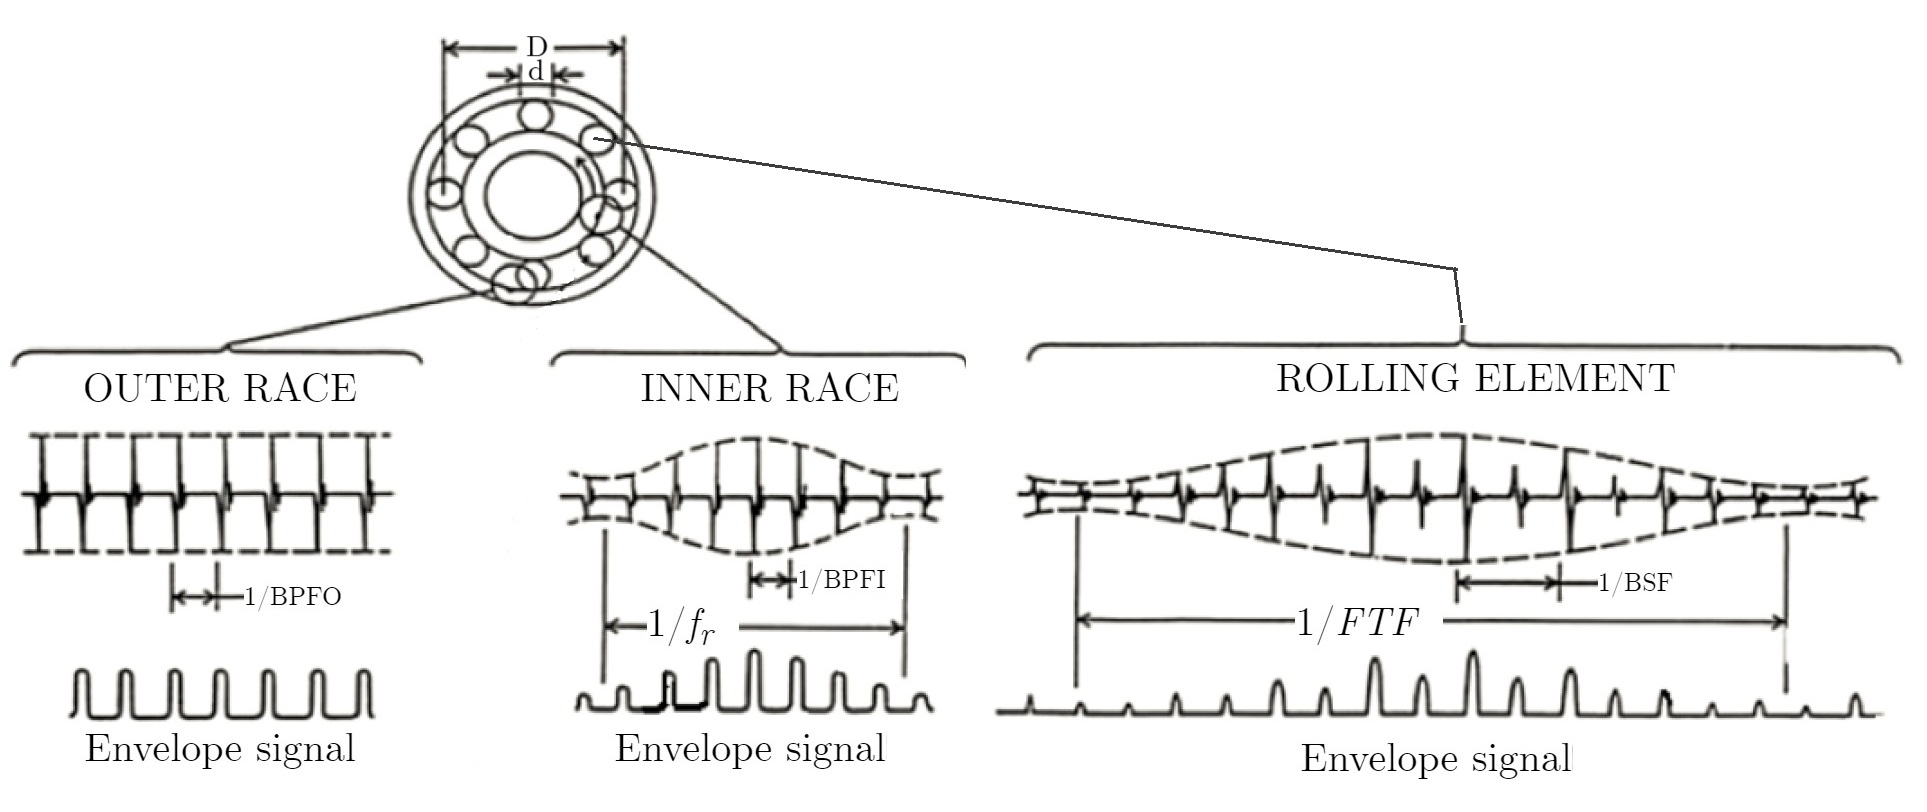
\includegraphics[width=\textwidth]{images/StateArt/bearing.jpg}
    \caption{Typical bearing fault signals \cite{RollingSignature}}
    \label{fig:bearing_faults}
\end{figure}

An automated method for bearing diagnosis has been developed by \cite{sawalhi2008semi}. The method is parametric and can be adapted to a large variety of cases. In the study, it has been tested on a helicopter gearbox, a high speed ($\approx 12000$rpm) test bench application and a low speed ($\approx 1800$rpm) radar tower. 

The automated procedure \cite{sawalhi2008semi} has been extended by a more recent study \cite{schlechtingen2019automated} where the authors applied a Cepstral Editing Procedure (\gls{cep}) based signal Pre-Whitening (\gls{pw}). The \gls{glo:frmwrk} has been tested on data collected from seventeen wind turbines. The procedure was successful in this case study, the preprocessing flow applied to the time-series, and the resulting spectral in which the \gls{bpfi} is exploited to detect the fault, are shown in \autoref{fig:turbine_faults}.

\begin{figure}
    \centering
    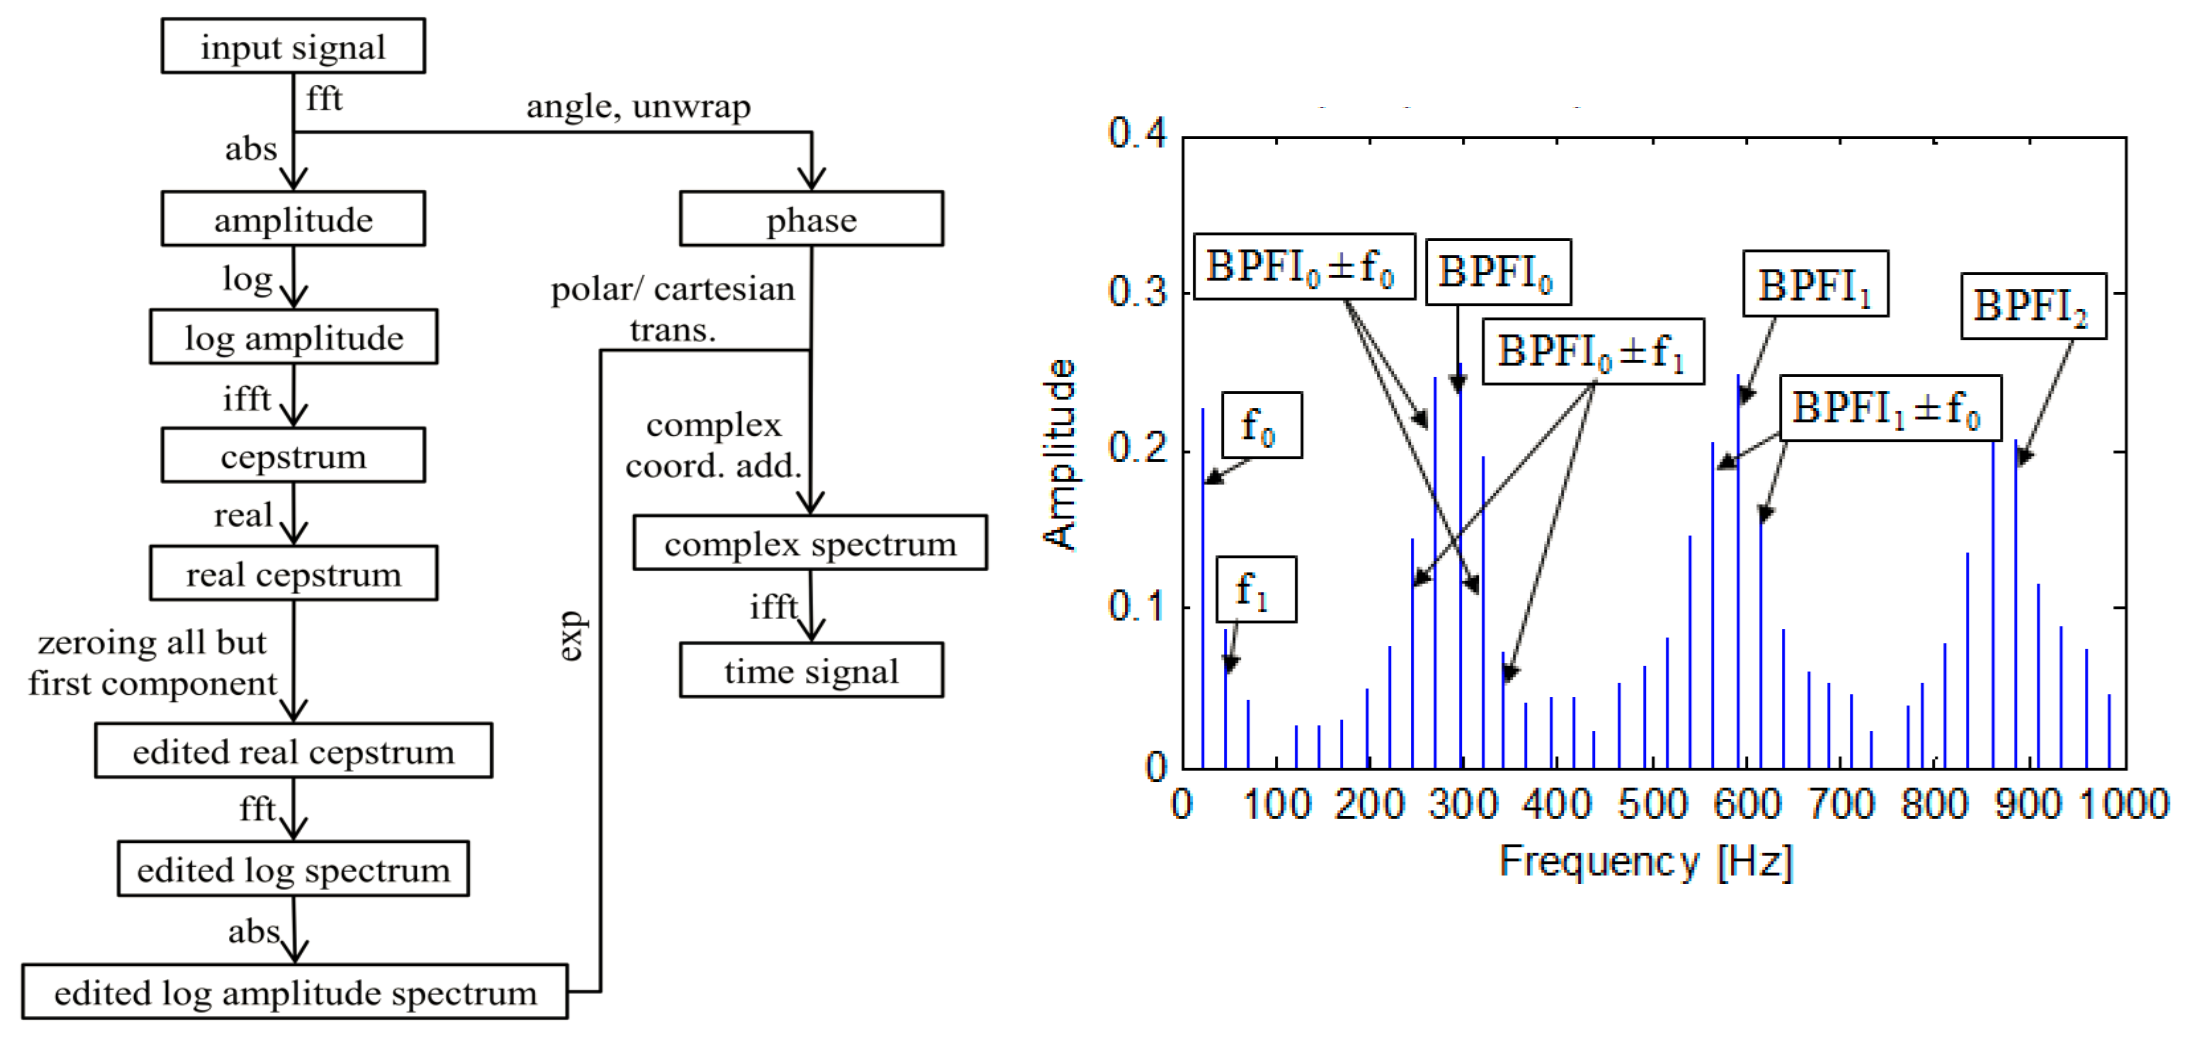
\includegraphics[width=\textwidth]{images/StateArt/spectrum.png}
    \caption{Preprocessing schematic and spectrum of a bearing fault signal \cite{schlechtingen2019automated}}
    \label{fig:turbine_faults}
\end{figure}

\subparagraph*{Novelty detection}
As anticipated, most of the time there is almost no precise knowledge about the physics of the system and data collections about faults are not available. In this case, \emph{novelty detection} (\gls{nd}) can be used. The task of detecting if a condition is \quoted{novel} can be seen as a classification problem with only one class (the data collected on the healthy system). The general idea is that if the one-class classifier is not able to classify a new observation as \quoted{healthy}, it means that the observation is \quoted{novel}.

Once the novelty detection algorithm is trained, it can be used to give an estimate of \quoted{how novel} the current behaviour of the system is. One of the major issues with \gls{nd} is to set the threshold value to decide if the observation is novel or not \cite{NoveltyReview}. This is because the value of the metric is hardly linkable to a physical property, and the span of the metric is not known a priori.

In \autoref{tab:novelTechniques}, the novelty detection techniques described in the comprehensive review \cite{NoveltyReview} are summarized. The review makes clear that in the field of \gls{nd}, both supervised and unsupervised techniques are used. It categorize the techniques into:
\begin{itemize}
    \item \textbf{Probabilistic} - involves a density estimation of the data;
    \item \textbf{Distance-based} - are the class of \gls{glo:clust}ing techniques used traditionally for classification;
    \item \textbf{Reconstruction-based} - use a regression model to reconstruct the data, then the error is used to detect the novelty;
    \item \textbf{Domain-based} - try to define a boundary that contains all the normal data;
    \item \textbf{Information-theoretic} - is based on the idea that novel data significantly alter the information content of the dataset.
\end{itemize}

{% \usepackage{tabularray}
\begin{longtblr}[
    caption = {State of the Art techniques for \gls{nd} \cite{NoveltyReview}},
    label = {tab:novelTechniques},
  ]{
    row{2} = {t},
    row{3} = {t},
    row{5} = {t},
    row{6} = {t},
    row{7} = {t},
    row{8} = {t},
    row{9} = {t},
    row{10} = {t},
    hline{1,11} = {-}{0.08em},
    hline{2} = {-}{},
  }
  \textbf{Model} & \textbf{Type}\\
  Mixture models & probabilistic, parametric\\
  State-space models & probabilistic, parametric\\
  Kernel density estimators & probabilistic\\
  Nearest neighbour & distance-based\\
  Clustering & distance-based\\
  Neural networs & reconstruction-based\\
  Subspace-based approaches~ & reconstruction-based\\
  Support vector descriptors & domain-based\\
  One-class support vectors & domain-based
  \end{longtblr}}

The first two terminologies are adopted also in the technical review of \gls{nd} methods \cite{NoveltyTech}. This study also categorizes the pattern to be identified in the following classes:
\begin{itemize}
    \item \textbf{Point pattern} - are single instances that are anomalous \gls{wrt} the rest of the data;
    \item \textbf{Contextual patter} - are anomalous \gls{wrt} a specific context;
    \item \textbf{Collective pattern} - is a collection of data instances that are anomalous if considered together.
\end{itemize}

The three distinct concepts are illustrated in \autoref{fig:pattern_types}.

The task of detecting the novelty is often associated with the task of predicting the \gls{glo:rul} (\gls{rul}) before the fault becomes fatal for the component.

\begin{figure}
    \centering
    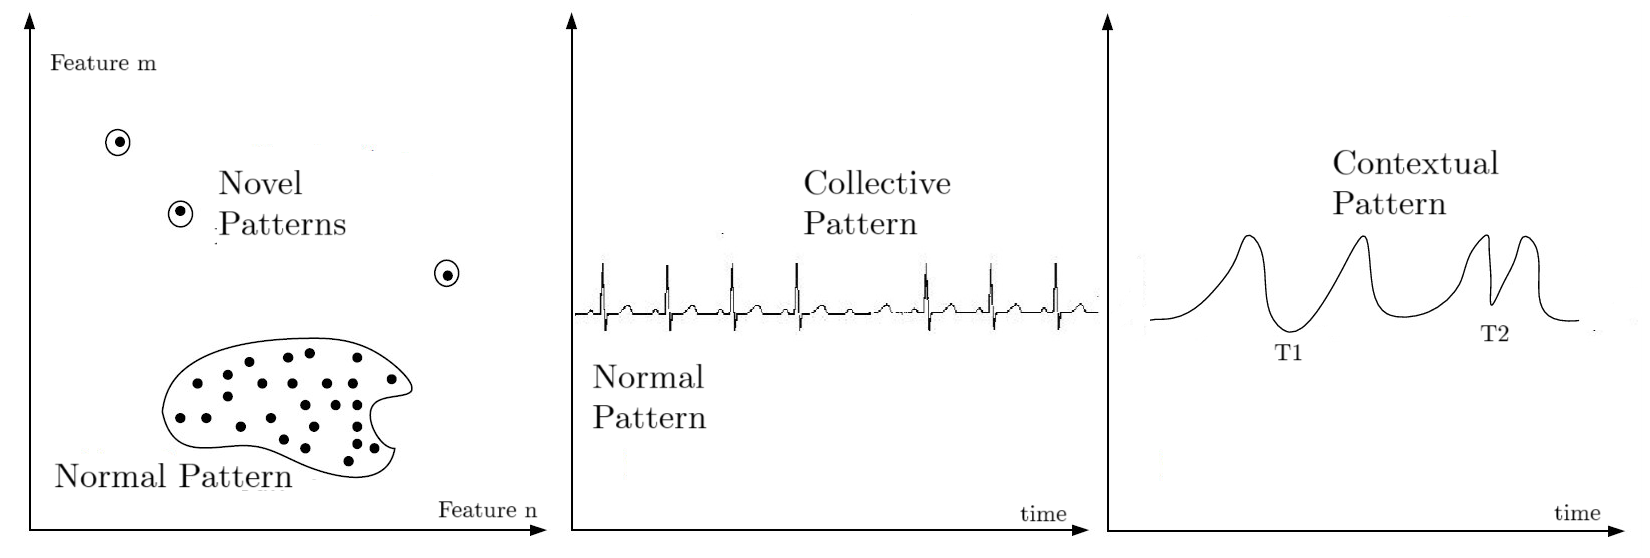
\includegraphics[width=\textwidth]{images/StateArt/patterns.png}
    \caption{Types of patterns \cite{NoveltyTech}}
    \label{fig:pattern_types}
\end{figure}

A novel \gls{glo:frmwrk} for performing \gls{nd}, \gls{fd} and \gls{rul} predictions has been proposed by researchers at PIC4SeR\footnote{\url{https://pic4ser.polito.it/}} \cite{Umberto}. It is based on several autonomous agents working together on a database.  The authors aimed to perform \gls{pdm} in a scenario in which there is no physical knowledge and no prior data collections about the maintained system. The \gls{glo:frmwrk} is meant to be set in a \emph{training phase} on a new machine, to collect the \emph{normal} data and train the \gls{ml} model. After that, it will continuously work in \emph{testing mode}: the \gls{glo:frmwrk} will compute a prediction error on the current data that is used as a novelty metric.

The \gls{glo:feature}s are pre-processed using a windowing function and a cumulative absolute sum. Three regression models are used to perform \gls{nd} and \gls{fd}: a Linear Regressor \gls{lr}, a Decision Tree (\gls{dt}) and a Random Forest (\gls{rf}). The user of the \gls{glo:frmwrk} can decide which regressor to use in each specific case. 

The model can be retrained after a novelty has been detected, to update the model with the new data. Even if the \gls{glo:frmwrk} is meant to be trained on a new machine, it can be used also on a machine that has been in service for years: the faults already present will be part of the training database, but the predictions will still be useful because of the tendency of the faults to worsen over time.

The \gls{rul} predictions are made by averaging the prediction error in two intervals and then performing a linear regression on the two points. 

This \gls{glo:frmwrk} has been successfully tested on:  
\begin{itemize}
    \item a synthetic dataset that the authors created to emulate a bearing fault (using the definitions of the 4 typical faults \cite{RollingSignature}).
    \item a real dataset of bearing faults provided by the Center for Intelligent Maintenance Systems \cite{IMSpaper}
    \item a laboratory test on spring probes
\end{itemize}

In the first two cases, the \gls{glo:frmwrk} was able to detect the novelty and predict the \gls{rul}, in the laboratory test, it was able to recognise the new data as \emph{healthy} because the probes were not yet damaged. The graphical results of one test on real-world data are shown in \autoref{fig:umbertoresult}.

\begin{figure}
    \centering
    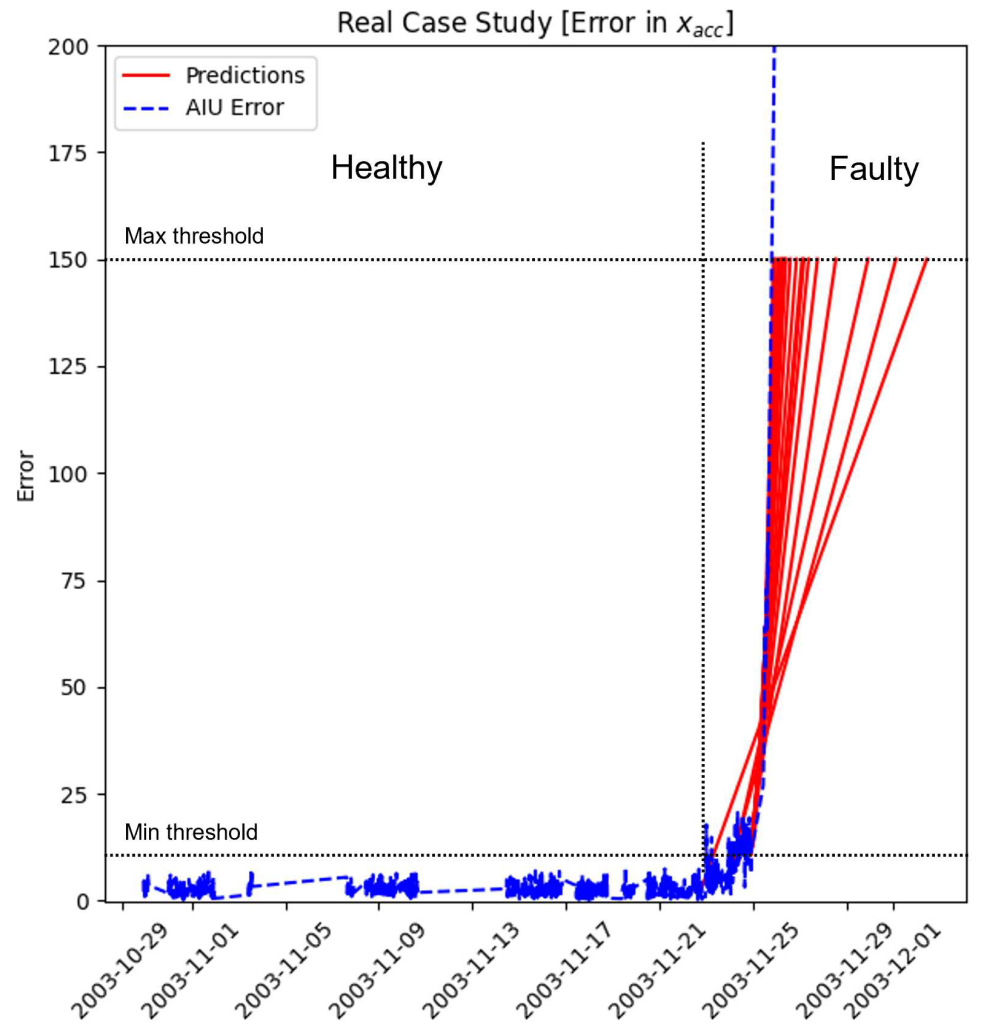
\includegraphics[width=0.6\textwidth]{images/IMS/UmbertoResults.png}
    \caption{Results provided by \cite{Umberto} for the test $\text{n}^\circ$1 of \gls{ims} dataset.}
    \label{fig:umbertoresult}
\end{figure}


\paragraph*{Clustering}
The most common unsupervised task is \gls{glo:clust}ing. In recent years, the volume of data collected in a typical factory has increased dramatically. Clustering is a collection of tools to extract information from huge amounts of unlabeled data. 

These algorithms can be divided into: \emph{partitioning-based} where the task is to define the boundaries between the \gls{glo:clust}s; \emph{hierarchical-based} that shows the relation between each pair of \gls{glo:clust}s depending on the medium of similarity or dissimilarity; \emph{density-based} that describes the \gls{glo:clust}s as a dense region of data points separated by low-density regions; \emph{grid-based} that apply the transformation of the \gls{glo:feature} space into a grid before proceeding with the \gls{glo:clust}ing and \emph{model-based} that use a statistical or deep-learning model to describe the data.

Recently, the survey \cite{Abla2019survey} provided a comprehensive overview of the most common \gls{glo:clust}ing algorithms used in an industrial context, with reference studies. The comparison of the study is reported in \autoref{tab:clustcomparison}.

{\small% \usepackage{color}
% \usepackage{tabularray}
\begin{longtblr}[
    caption = {Clustering algorithms comparison \cite{Abla2019survey}. $n$ = number of samples, $k$ = number of clusters, $d$ = number of features.},
    label = {tab:clustcomparison},
  ]{
    cell{2}{1} = {t},
    cell{2}{2} = {t},
    cell{3}{1} = {t},
    cell{3}{2} = {t},
    cell{5}{1} = {t},
    cell{5}{2} = {t},
    cell{6}{1} = {t},
    cell{6}{2} = {t},
    cell{7}{1} = {t},
    cell{7}{2} = {t},
    cell{8}{1} = {t},
    cell{8}{2} = {t},
    cell{9}{1} = {t},
    cell{9}{2} = {t},
    cell{10}{1} = {t},
    cell{10}{2} = {t},
    hline{1,23} = {-}{0.08em},
    hline{2} = {-}{},
  }
  \textbf{Algorithm} & \textbf{Volume} & {\textbf{High}\\\textbf{dim.}} & {\textbf{Cluster}\\\textbf{shape}} & \textbf{Complexity} & \textbf{n. param.}\\
  K-means & any & no & non-convex & $\mathcal{O}(nkd)$ & 1\\
  K-modes & large & yes & non-convex & $\mathcal{O}(n)$ & 1\\
  K-medioids & small & yes & non-convex & $\mathcal{O}(n^2dt)$ & 1\\
  PAM & small & no & non-convex & $\mathcal{O}(k(n-k)^2)$ & 1\\
  CLARA & large & no & non-convex & $\mathcal{O}(k(40+k)^2+$&1\\
  &&&&$+k(n-k))$ & \\
  Ward & any & no & non-convex & $\mathcal{O}(n)$ & 1\\
  BIRCH & large & no & non-convex & $\mathcal{O}(n)$ & 2\\
  CURE & large & yes & any & $\mathcal{O}(n^2\log n)$ & 2\\
  ROCK & large & no & any & $\mathcal{O}(n^2+n^2 \log n)$ & 1\\
  Chamelon & large & yes & any & $\mathcal{O}(n^2)$ & 3\\
  \gls{dbscan} & large & no & any & $\mathcal{O}(n \log n)$ & 2\\
  OPTICS & large & no & any & $\mathcal{O}(n \log n)$ & 2\\
  DENCLUE & large & yes & any & $\mathcal{O}(D)$ & 2\\
  Wavecluster & large & no & any & $\mathcal{O}(n)$ & 3\\
  STING & large & no & any & $\mathcal{O}(k)$ & 1\\
  CLIQUE & large & yes & any & $\mathcal{O}(ck+mk)$ & 2\\
  OPTGRID & large & yes & any & $\mathcal{O}(nd \log n)$ & 3\\
  \gls{em} & large & yes & non-convex & $\mathcal{O}(knp)$ & 3\\
  COBWEB & small & no & non-convex & $\mathcal{O}(n^2)$ & 1\\
  \gls{som} & small & yes & non-convex & $\mathcal{O}(n^2m)$ & 2\\
  \end{longtblr}}